\documentclass[]{article}
\usepackage[utf8]{inputenc}
\usepackage{pdfpages}
\usepackage{amsmath}
\usepackage{amssymb}
\usepackage{graphicx}
\usepackage{geometry}
\usepackage{enumitem}
\usepackage{amsthm}
\usepackage{stmaryrd}
\usepackage{mathtools}
\usepackage{mathrsfs}

\geometry{hmargin=2cm}

% Environnement type théorème
\newtheorem{mythm}{Théorème}
\newtheorem{myproposition}{Proposition}
\newtheorem{myproperty}{Propriété}
\newtheorem{mylemma}{Lemme}
\newtheorem{mycoro}{Corollaire}

% Environnement type texte
\theoremstyle{remark}
\newtheorem{mynot}{Notation}
\newtheorem{myrem}{Remarque}
\newtheorem{myexer}{Exercice}
\newtheorem{myproof}{Preuve}
\newtheorem{myexmpl}{Exemple}

% Environnement de définition
\theoremstyle{definition}
\newtheorem{mydef}{Définition}
\newtheorem{myquestion}{Question}

\setlist[itemize]{label=-}

% Carré de fin de preuve
\newcommand{\cqfd}{
	\hfill$\square$
}

% Définition de fonction
\newcommand{\func}[5]{
#1 ~ : ~ \left\{ \begin{array}{lcl}
	#2 & \longrightarrow & #3 \\
	#4 & \longmapsto & #5
\end{array}
\right.
}

\newcommand{\fun}[3]{
#1 ~ : ~ #2 \longrightarrow #3
}

\newcommand{\funcinline}[5]{
	#1 \, : \, #2 \longrightarrow #3, ~ #4 \longmapsto #5
}

\newcommand{\funcshort}[3]{
	#1 \, : \, #2 \longrightarrow #3
}

\newcommand{\anonfunc}[4]{
	\left\{ \begin{array}{lcl}
		#1 & \longrightarrow & #2 \\
		#3 & \longmapsto & #4
	\end{array}
	\right.
}

\newcommand{\vect}{\text{Vect}}

\newcommand{\card}{\text{Card }}

\newcommand{\DS}{\displaystyle}

\begin{document}
	\part{Analyse du signal}
	\section{L'analyse de Fourier}

	\paragraph*{}
En termes d'analyse du signal, l'utilisation de l'analyse de Fourier parait être indispensable. Le principe sous-jacent à cette analyse provient de l'étude des Séries de Fourier, qui permet sous certaines conditions de décomposer un signal périodique en une somme de signaux sinusoïdaux de même fréquence et de fréquences harmoniques. 

Nous allons étudier les outils sur lesquels reposent cette analyse, puis observer l'application sur des exemples, qui mettront en valeur les limites de ce procédé et la nécessité d'utiliser une analyse plus poussée comme l'analyse en ondelettes. Cette partie sera limitée aux fonctions d'une seule variable. 

	
	\subsection {Séries de Fourier}
		Dans cette partie, nous voulons d'abord étudier le cas des fonctions de $L^2(\mathbb{T})$. On verra que dans cet espace fonctionnel, il existe une base dans laquelle n'importe quelle fonction peut être décomposée de manière unique. De plus, il sera important de prendre en compte la notion de convergence de cette décomposition qui est nécessaire dans de nombreuses applications. 

		On se restreint aux fonctions $2\pi$-périodiques, car l'étude des autres fonctions périodiques reste la même à des coefficients multiplicatifs près. 	
		
			
		\begin{mydef} 
			
			On munit $L^2(\mathbb{T})$ d'un produit scalaire et de sa norme induite, définis par : 
			
			
			$$ \langle f,g \rangle = \frac{1}{2\pi} \int_{0}^{2\pi} f(t) \overline{g(t)} dt$$
				
			$$ \| f \|_2 =  \left( \frac{1}{2\pi} \int_0^{2\pi}| f(t) |^2 dt\right)^{\frac{1}{2}}$$	
				
		\end{mydef}		 
		 
		 Il s'agit ainsi d'un espace de Hilbert.
		 
		\begin{mydef}
			On définit pour tout $k \in \mathbb{Z}$,  $e_k(t):=e^{ikt}, \quad t\in \mathbb{R}.$	
		\end{mydef}
		
		Ces fonctions sont aux polynômes trigonométriques ce que les puissances de l'indéterminée sont aux polynômes classiques.
		
		\begin{mydef}
			Soit $f$ une fonction de $L^2(\mathbb{T})$ et $N$ un entier positif, on définit sa $N$-ième série de Fourier par
			
			\begin{align*}
				S_N(f) &= \sum_{k = -N}^N c_k(f) e_k \\
				&= \sum_{k = -N}^N \langle f, e_k \rangle e_k
			\end{align*}
			
			où $c_k$ est le $k$-ième coefficient de Fourier de $f$.
		\end{mydef}

		La $N$-ième série de Fourier d'une fonction $f$ est sa projection orthogonale sur l'espace engendré par $e_{-N}, e_{-N+1} \cdots e_N$. On retrouve une propriété intuitive des projections orthogonales, qui porte ici le nom d'inégalité de Bessel :
		
		\begin{mythm}
			Soit $f \in L^2(\mathbb{T})$, on a pour tout $N$, $\|S_N(f)\|_2 \leqslant \|f\|_2$
		\end{mythm}
		
		\begin{myproof}
			\begin{align*}
				\| f - S_N(f) \|^2_2 &= \langle f - S_N(f), f -S_N(f) \rangle \\
									 & = \| f \|^2_2 + \| S_N(f)\|^2_2 + \langle f, S_N(f) \rangle + \langle S_N(f), f \rangle \\ 
									 & = \| f \|^2_2 + \| S_N(f)\|^2_2 + \langle f, S_N(f) \rangle + \overline {\langle  f, S_N(f)\rangle } \\
									 &= \| f \|^2_2 + \| S_N(f)\|^2_2 - 2Re (\langle f, S_N(f) \rangle) \quad \text{ car } \langle f, S_N(f) \rangle = \| S_N(f)\|^2 \\
									 &=  \| f \|^2_2 - \| S_N(f)\|^2_2
			\end{align*}
			
			$\| f \|^2_2 - \| S_N(f)\|^2_2 \geqslant 0$, d'où le résultat.
			\cqfd
		\end{myproof}
			On remarque également que si $P$ est un polynôme trigonométrique, alors $S_N(P) = P$ pour $N = \deg P$. 
			
			\begin{myproposition}
				$ (e_k)_{k\in\mathbb{Z}} $ est une base hilbertienne.
			\end{myproposition}
			
			\begin{myproof}	
				On cherche à montrer qu'il s'agit d'une famille orthonormée et dont les combinaisons linéaires sont denses dans $L^2 (\mathbb{T})$. Plus précisément, qu'elle est orthonormée et que pour tout $f \in L^2(\mathbb{T})$
				
				$$\lim\limits_{n \to \infty} \sum_{k = -n}^n \langle f, e_k \rangle e_k = f \quad (\text{dans } L^2(\mathbb{T}), \|\cdot\|_2)$$
				
				Soient $k, l \in \mathbb{Z}$, si $k=l$
				\begin{align*}
					\langle e_k, e_l \rangle = \|e_k\|_2^2 &= \frac{1}{2\pi}\int_0^{2\pi} e_k(t)\overline{e_k(t)}dt\\
					&  =  \frac{1}{2\pi}\int_0^{2\pi} e^{ikt}e^{-ikt}dt\\
					& = \frac{1}{2\pi} \int_0^{2\pi} 1 dt\\
					& = 1
				\end{align*}
				 
			
				Sinon, 
				\begin{align*}
				\langle e_k, e_l\rangle_2 & = \frac{1}{2\pi} \int_0^{2\pi} e_k(t) \overline{e_l(t)}dt 
				\\ & = \frac{1}{2\pi} \int_0^{2\pi}e^{ik t} e^{-il t} dt 
				\\ & = \frac{1}{{2\pi}} \int_0^{2\pi} e^{i(k-l)t} dt 
				\\ & = \frac{1}{{2\pi}}  \left[ \frac {e^{i(k-l) t}} {{i(k-l)}} \right] _0^{2\pi}
				\\ & = \frac {e^{i (l-k){2\pi}} - e^{i(l-k)  0}} {i {2\pi}(l-k)}
				\\ & = \frac {1 - 1}{i {2\pi}(l-k)}\\
				&= 0
				\end{align*}

				Montrons à présent que toute fonction de $L^2(\mathbb{T}) $ admet une décomposition unique dans cette base.
				
				Soit $f \in L^2(\mathbb{T})$ et $\varepsilon > 0$, sachant que les fonctions $2\pi$-périodiques continues sont denses dans $L^2(\mathbb{T})$, il existe $f_0$ continue et $2\pi$-périodique telle que $\forall t, ~ | f(t) - f_0(t)| < \varepsilon$. 
				
				Celle-ci étant périodique, on en déduit l'existence de $F_0$ définie sur le cercle unité telle que $f_0(t) = F_0(e^{it})$.
				
				D'après le théorème de Stone-Weierstrass, il existe un polynôme trigonométrique $P$ tel que $\forall t,  ~ |f_0(t) - P(e^{it})| < \varepsilon $.
				Par l'inégalité triangulaire, on a:
				\begin{align*}
					\| S_N(f) -f \|_2 &\leqslant \|S_N(f) - S_N(P)\|_2 + \| S_N(P) - P \|_2 + \| f- P \|_2 \\
				&	\leqslant 2 \| f - P\|_2 + \| S_N(P) - P\|_2 \quad \text{par l'inégalité de Bessel} \\
				& \leqslant 2 \| f - P\|_2 \quad \text{ pour } N\geqslant \deg(P) \\
				& \leqslant 2 \| f - f_0\|_2 + 2 \| f_0- P\|_2 \\
				& \leqslant 4 \varepsilon
				\end{align*}
				\cqfd
				
			\end{myproof}
			
		Comme cette famille est une base Hilbertienne de $L^2(\mathbb{T})$, il est donc possible de décomposer les fonctions de cet espace dans cette base de manière unique. C'est à dire que:
				$$ \lim_{N\to +\infty} \|S_N(f) -f \|_2 = 0 $$
				
		On dit que la convergence est en moyenne quadratique. 

	Il est possible d'étendre l'analyse en séries de Fourier pour les fonctions périodiques de $L^1(\mathbb{T})$, tout en conservant une notion de convergence. 
	
	\begin{mythm}
		Soit $f \in L^1(\mathbb{T})$. Si ses coefficients de Fourier forment une famille sommable, $(c_n(f))_{n\in\mathbb{Z}} $, alors: 
		$$ \lim_{N\to +\infty} \|S_N(f) -f \|_{L^\infty(\mathbb{T})} = 0 $$ 
		Et $f$ admet un représentant continu. 

	\end{mythm}
			
	\begin{myproof}

		$S_N(f)$ converge normalement (vers une limite continue): 
		$$ \sum_{p \in \mathbb{Z}} \|c_p(f)e_p\|_\infty = \sum_{p \in \mathbb{Z}} |c_p(f)| < \infty $$
		$S_N(f)$ converge pour la norme $\| \cdot \|_\infty $ et donc pour $\| \cdot \|_{L^{\infty}} $.
		Par injection continue de $L^\infty(\mathbb{T})$ dans $L^2(\mathbb{T})$, $S_N$, sa limite dans $L^\infty(\mathbb{T})$ coïncide avec $f$ (sa limite dans $L^2(\mathbb{T})$). Donc $f$ admet bien un représentant continu. 
		
		\cqfd
	\end{myproof}
	
	
			
	Au delà de l'existence d'une convergence, il peut-être utile d'étudier la vitesse de convergence. Il s'agit d'étudier la décroissance des coefficients de Fourier d'une fonction. 
	
	\begin{mythm}
		Soit $f$ une fonction de classe $\mathcal{C}^k$. Alors, $c_p(f^{(k)}) = (ip)^kc_p(f)$ et il existe une constante $C$ telle que:
			$$ | c_p(f) | \leqslant \frac{C}{|p|^k} $$
	\end{mythm}
	
	\begin{myproof}
		Par récurrence sur $k$. 
		pour $k=1$, on a :
			\begin{align*}
			c_p(f') &= \frac{1}{2\pi}\int_0^2\pi f(t)e^{-ipt}dt \\
					&= -\frac{1}{2\pi}\int_0^2\pi f(t)(-ip) e^{-ipt}dt + \frac{1}{2\pi}\left[f(t)e^{-ipt} \right]_0^{2\pi} \\
					& = \frac {ip}{2\pi} \int_0^2\pi f(t)e^{-ipt}dt \\
					& = \frac {ip}{2\pi} c_p(f)
			\end{align*}
			Et on conclut par récurrence sur $k$.
		
		De plus, 
		\begin{align*}
		|c_p(f^{(k)})| &\leqslant \frac{1}{2\pi}\int_0^{2\pi}|f^{(k)}(t)|dt \\
		& \sup_{[0, 2\pi]} |f^{(k)}(t)| =: C 
		\end{align*}
		Donc $ \DS|c_p(f)| = \frac {|c_p(f^{(k)})|}{|p|^k} \leqslant \frac{C}{|p|^k} $.
		\cqfd		
	\end{myproof}
		
	
	\newpage
	
	\begin{myexmpl}
		Étudions la décomposition en séries de Fourier de la fonction en créneaux définie par: 
		$$ f(x) = \left\{
		\begin{array}{cc}
			-1 & \text{ sur }[-\pi, 0[ \\
			1 & \text{ sur }[0, \pi[ \\
		\end{array}
		\right. $$
	
	[CALCULS ICI]
	
	\begin{figure}[h]
		\centering
		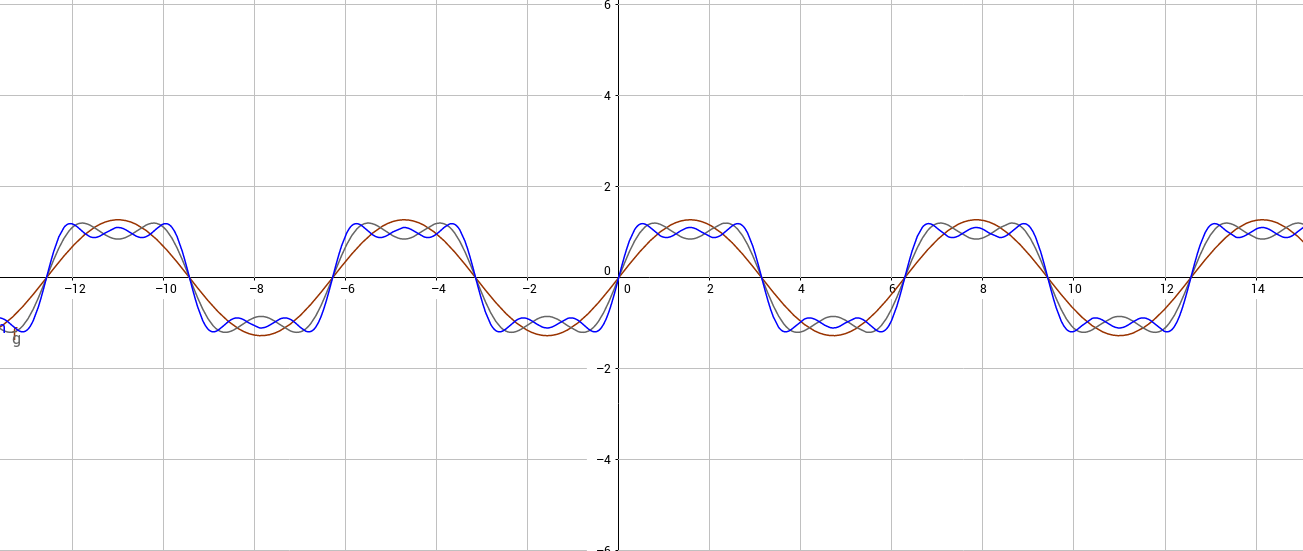
\includegraphics[width=350pt]{Signal_carre_fourier.png}
		\caption{Une image de voiture pour trois résolutions différentes}
	\end{figure}
	
	\end{myexmpl}
	
	\subsection{Transformée de Fourier}
		La transformée de Fourier permet d'étendre les notions abordées dans le cadre des séries de Fourier dans un cadre plus général, notamment pour des fonctions non périodiques. 
		Dans ce cadre, on ne peut plus se restreindre à la famille des $e_k$ définie précédemment, car la notion de pulsation n'est plus valable dans ce cadre. 
	
	\begin{mydef}
		Soit $f(t)$ une fonction de $L^1(\mathbb{R})$ à valeurs réelles ou complexes. La Transformée de Fourier est une fonction complexe définie par :
		$$ \mathcal{F}[f(t)] = F(k)= \int_{-\infty}^{+\infty}f(t)e^{-ikt}dt $$ 
	\end{mydef}

	\begin{myrem}
		La condition que la fonction $f(t)$ soit intégrale est suffisante pour que l'intégrale soit bien définie et que la transformée de Fourier existe. 
		De plus, $F(k)$ sera une fonction continue et bornée qui tend vers 0 lorsque $|k| \longrightarrow \infty$.
		
		En effet, $|f(t)e^{-i k t}| \leqslant |f(t)|$ et à $t$ fixé $k \mapsto f(t) e^{- i k t}$ est continue.
	\end{myrem}
	
	\begin{myproof}
		PREUVE DE RIEMANN-LEBESGUE
	\end{myproof}
	
	Nous pourrons nous restreindre aux fonctions de $L^1$ pour cette étude. 
	Comme pour l'étude des séries de Fourier, une notion très importante est de pouvoir reconstruire le signal à partir de sa transformée de Fourier. Pour ce faire, il est possible d'utiliser la transformée de Fourier inverse. 

	\begin{mydef}
		En ajoutant la condition que $f(t)$ soit continue aux conditions précédentes, on peut définir la transformée de Fourier inverse par :
		$$ \overline{\mathcal{F}}[F(k)] = f(t)=\frac{1}{{2\pi}} \int_{-\infty}^{+\infty}F(k)e^{ikt}dt $$ 
	\end{mydef}
	
	\begin{myrem}
		Si la condition de la continuité de $f(t)$ n'est pas respectée, la transformée de Fourier de $f(t)$ sera quand même définie, mais l'égalité entre $f(t)$ et $\overline{\mathcal{F}}[\mathcal{F}[f(t)]]$ ne sera vérifiée que presque partout. 
	\end{myrem}
			
	\subsubsection{exemple}
	[exemple de deux signaux successifs, l'un défini sur $ ] -\infty; 0[$ et l'autre sur $ [0; +\infty[$ qui ont la même décomposition en spectre que s'ils avaient été simultanés]
	
	\subsection{Transformée de Fourier à fenêtre glissante}
	La transformée de Fourier à fenêtre glissante est une solution par rapport au problème de la notion de temporalité apporté par l'étude de signaux continus et non plus périodiques. 

	En reprenant la définition de la transformée de Fourier précédente, on peut l'étendre pour ajouter la notion de fenêtre glissante. 
		
	\begin{mydef}
		Soit $f(t)$ une fonction qui possède une transformée de Fourier. On peut définir la Transformée de Fourier à fenêtre glissante par :
		$$ F(k, \tau)= \int_{-\infty}^{+\infty}f(t)e^{-ikt} \overline{w(t - \tau)}dt$$
		où $w(t)$ est la fonction de fenêtre, et $\tau$ le paramètre de translation. 
	\end{mydef}
	Il s'agit ensuite de trouver le format de fenêtre adéquat. 
	
	\subsubsection{exemple}
	[Reprendre l'exemple précédent en montrant que ca fonctionne bien, puis faire un autre exemple, comme la fonction en créneau et montrer que ca ne suffit pas pour les discontinuités]
	
	
	\subsection{Transformée de Fourier discrète}
			
	Ces conditions sont nous permettent de définir un cadre pour utiliser la transformée de Fourier. Néanmoins, lors d'applications à l'informatique, nous ne pouvons pas conserver une infinité de valeurs, et il est nécessaire de pouvoir travailler sur des valeurs discrètes, tout en conservant au plus les propriétés pour décomposer et recomposer les fonctions. 		
	Dans le cadre de la transformée de Fourier discrète, au lieu d'utiliser des fonctions, nous allons nous intéresser à des suites qui correspondront à l'échantillonnage de la fonction. Il est important de noter que ces suites seront finies, pour correspondre à l'espace de stockage fini des ordinateurs. 
	

	\begin{mydef}
		On définit la fréquence d'échantillonnage comme le nombre d'échantillons par unité de temps.  
	\end{mydef}
		Pour que l'échantillonnage soit suffisant pour obtenir une reconstitution de qualité suffisante, on peut se référer au théorème de Nyquist-Shannon. 
		
	\begin{mythm}
		Si une fonction $f(t)$ ne contient pas de fréquences plus élevées que $B$ Hz, il est complètement décrit en donnant une suite de ses valeurs a des points régulièrement espacés tout les $\frac{1}{2B}$ secondes.
	\end{mythm}
	
	Dans la mesure où tous les appareils utilisés pour enregistrer des signaux ne peuvent pas capter de valeurs infinies, il sera possible de reconstituer le signal à partir de cette suite de valeurs, avec pour limite la qualité des appareils d'enregistrements et non pas les outils mathématiques. Dans certains cas, l'acuité humaine peut également servir de limite.
	
	\begin{myexmpl}
		 Pour les enregistrements audios, la fréquence d'échantillonnage des fichiers pour le format CD est traditionnellement de 44 100 Hz, ce qui est juste supérieur au double de la fréquence la plus élevée que peut percevoir l'oreille humaine en théorie, c'est à dire 20 000 Hz. 
	\end{myexmpl}
	
	\begin{mydef}
			On considère une suite $(s_n)_{n\in \{0; N -1 \}}$ de N termes. La transformée de Fourier Discrète permet d'obtenir la suite  $(S_n)_{n\in \{0; N -1 \}}$ de N termes définis par :
			$$ S_k = \sum_{k=0}^{N-1}s_n e^{-2i\pi k\frac{n}{N}} $$
	\end{mydef}
		De la même manière que pour la transformée de Fourier, on pourra également définir la transformation inverse.
		
	\begin{mydef}
		Dans les mêmes conditions que ci dessus, on définit la transformée de Fourier discrète inverse par :
			$$ s_n =\frac{1}{N} \sum_{k=0}^{N-1}S_k e^{2i\pi k\frac{n}{N}} $$
	\end{mydef}
	
	Ces transformations sont sans pertes d'informations, ainsi, si les conditions du théorème de Nyquist-Shannon sur la fréquence d'échantillonnage ont été respectées, alors le signal peut être reconstitué sans perte via ces transformations successives. 
	
	L'avantage de l'utilisation de la transformée de Fourier discrète se retrouve également dans la vitesse d'exécution des calculs. En effet, la transformée de Fourier continue à une complexité en $O(N^2)$ alors qu'il existe des algorithmes comme celui de La transformée de Fourier rapide, qui sous certaines conditions sur le nombre de termes de la suite à transformer, peuvent atteindre une complexité en $O(n\log(n))$.
\end{document}
